\documentclass{article}
\usepackage{graphicx} % Required for inserting images
\usepackage{tikz}
\usetikzlibrary{arrows.meta, decorations.markings}
\usepackage{amsmath}
\usepackage{float}
\usepackage{circuitikz}

\title{Maxwell's Equations: A Step-by-Step Derivation}
\author{Varshaa Venkitesh}
\date{June 2025}

\begin{document}
\maketitle

\tableofcontents

\pagebreak
\section{Introduction}
Maxwell's equations are a set of four equations that describe the basic behavior of electromagnetic fields. By combining these equations, Maxwell was able not only to unify electricity and magnetism (previously considered completely separate physical phenomena) but also to establish that light itself is an electromagnetic wave.

\vspace{1em}

Maxwell's equations have been used to explain many real-world occurrences such as the behavior of electrical circuits and the propagation of EM waves such as light. They also allowed for the development of modern technologies such as the radio, television, and wireless communication.

\vspace{1em}

This article presents step-by-step mathematical derivations of Maxwell's equations, as well as exploring their geometric meaning and connection to physical intuition. This kind of approach is especially appropriate when studying Maxwell's equations because the relations that led to the equations were initially observed through experiments rather than derived through complex mathematics.

\vspace{1em}
One note before we begin: for the mathematical derivations, it would be helpful to have familiarity with or have taken a class in multivariable calculus. All the concepts required, however, are provided in the next section, "Mathematical Tools", for your reference. Also, when I use the closed integral sign $\oint$, it is typically simply to emphasize/remind that the path or surface we are integrating over is closed.

\pagebreak
\section{Mathematical Tools}

To understand Maxwell's equations and their derivations, it is crucial to grasp the following fundamental concepts: dot and cross products, differential operators, and vector calculus theorems.

\subsection{Vector Operations}
The dot product (AKA the inner product) and cross product are ways to multiply vectors. In these cases, we will define $\theta$ as the angle between the two vectors we are multiplying. By convention, the value of $\theta$ will be between 0 and 180 degrees, or, equivalently, between 0 and $\pi$ radians.
\subsubsection{Dot Product}
The dot product of two vectors $\vec u$ and $\vec v$ is: 
\begin{equation}
 \vec u \cdot \vec v = |\vec u||\vec v|cos\theta
\end{equation}
Note that the end result is a scalar quantity. Geometrically, the dot product gives the projection of one vector onto another.

\begin{center}
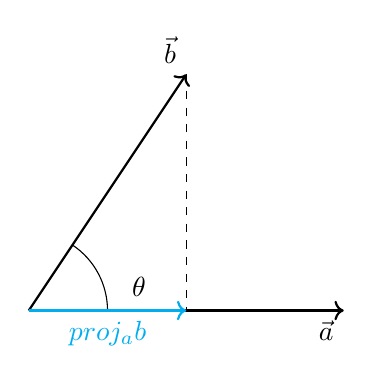
\begin{tikzpicture}[scale=2]
  % Vectors
  \draw[->, thick] (0,0) -- (2,0) node[anchor=north east] {$\vec{a}$};
  \draw[->, thick] (0,0) -- (1,1.5) node[anchor=south east] {$\vec{b}$};

  % Angle arc
  \draw (0.5,0) arc[start angle=0,end angle=56.3,radius=0.5];
  \node at (0.7,0.15) {$\theta$};

  % Projection line
  \draw[dashed] (1,1.5) -- (1,0);
  \draw[->, thick, cyan] (0,0) -- (1,0) node[midway, below] {$proj_a b$};
\end{tikzpicture}
\end{center}

\subsubsection{Cross Product}
The cross product of two vectors $\vec u$ and $\vec v$ is specific to two- or three-dimensional vectors:
\begin{equation}
 \vec u \times \vec v = |\vec u||\vec v|sin\theta
\end{equation}
This time, the end result is a vector quantity perpendicular to both $\vec u$ and $\vec v$, with direction determined by the right-hand rule. (Meaning, $\vec u \times \vec v = -(\vec v \times \vec u)$.) Geometrically, the magnitude of the cross product is the area of the parallelogram formed by the two vectors as its sides.

\begin{center}
\begin{tikzpicture}[scale=2]

  % Draw vectors
  \draw[->, thick] (0,0,0) -- (1,0,0) node[anchor=south] {$\vec{a}$};
  \draw[->, thick] (0,0,0) -- (0,1,0) node[anchor=west] {$\vec{b}$};

  % Cross product vector
  \draw[->, thick, purple] (0,0,0) -- (0,0,1) node[anchor=east] {$\vec{a} \times \vec{b}$};
\end{tikzpicture}
\end{center}

\subsubsection{Note on Dot vs. Cross Product Usage}
You have probably seen many physics formulas that either use the dot product or the cross product before, and you might wonder why a certain vector operation is being used for that formula. One way to figure out whether to use the dot or cross product for a certain formula is to think about when the effect is largest. For example, think about the formula for work. The most work is done when the force is going in the same direction as the object you are trying to move. So, we use the dot product ($W = \vec F \cdot \vec d = \vec F\vec dcos\theta$). Now think about the formula for torque. The most work is done when the force is perpendicular to the object you are trying to move (think of pushing on a door; you push perpendicular to the door hinge). So, we use the cross product ($\tau = \vec r \times \vec F = \vec r \vec F sin\theta$). 

\subsection{Differential Operators}

The vector differential operators are written using the nabla symbol (sometimes also called the del operator): 
\begin{equation}
\nabla = (\frac{\partial}{\partial x}, \frac{\partial}{\partial y}, \frac{\partial}{\partial z}) 
\end{equation}

\subsubsection{Gradient} %scalar field to vector
The gradient for function f(x,y,z) can be written as:
\begin{equation}
 \nabla f = \left( \frac{\partial f}{\partial x}, \frac{\partial f}{\partial y}, \frac{\partial f}{\partial z} \right)
\end{equation}
\subsubsection{Divergence} %vector field to scalar
The divergence of function f(x,y,z) can be written as: 
\begin{equation}
\nabla \cdot f = \frac{\partial f}{\partial x} + \frac{\partial f}{\partial y} + \frac{\partial f}{\partial z}
\end{equation}

\subsubsection{Curl} %vector field to vector
The curl of function f(x,y,z) = ($f_1$, $f_2$, $f_3$) can be written as:
\begin{equation}
\nabla \times f = det
  \begin{bmatrix}
    \hat{i} & \hat{j} & \hat{k}\\
    \frac{\partial}{\partial x} & \frac{\partial}{\partial y} & \frac{\partial}{\partial z}\\
    f_1 & f_2 & f_3
  \end{bmatrix}
  = \hat{i}(\frac{\partial f_3}{\partial y} - \frac{\partial f_2}{\partial{z}}) - \hat{j}(\frac{\partial f_3}{\partial x} - \frac{\partial f_1}{\partial{z}}) + \hat{k}(\frac{\partial f_2}{\partial{x}} - \frac{\partial f_1}{\partial y})
\end{equation}

\vspace{1em}

Note that the gradient and curl give a vector output, while the divergence results in a scalar.

\vspace{1em}

Each operator also carries a physical meaning. 

The gradient is a vector field that points in the direction of the local maximum of a function. Each vector in the gradient is where the function f increases at the fastest rate at that point.

Divergence describes sources and sinks. You can think about water (and this can be represented by arrows/vectors) flowing through a net at a specific rate. The divergence measures the net rate of change (with respect to time) of the water flowing out of the net. Specifically, if the amount of water flowing in is the same as the amount of water flowing out, the divergence is 0. Also, points at which the water tends to flow outward are called "sources", and points at which the water tends to flow inward are called "sinks". 

\vspace{3em}
\noindent
\begin{minipage}{0.4\textwidth} %minipages to make images side-by-side
\centering

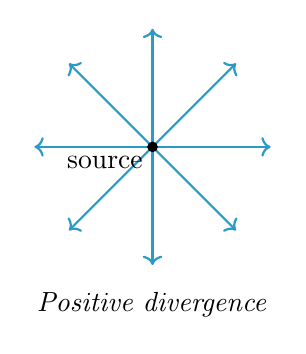
\begin{tikzpicture}
  \foreach \angle in {0,45,...,315} {
    \draw[->, thick, cyan!80!black] (0,0) -- (\angle:1.5);
  }
  \filldraw[black] (0,0) circle (0.06) node[below left] {source};
  \node at (0,-2) {\textit{Positive divergence}};
\end{tikzpicture}
\end{minipage} %don't put a blank space after this
\hfill %inserts spacing between the two minipages
\begin{minipage}{0.4\textwidth} %don't put a blank space before this
\centering
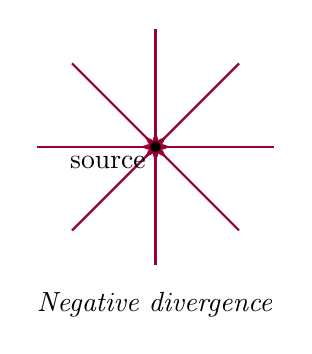
\begin{tikzpicture}
  \foreach \angle in {0,45,...,315} {
    \draw[<-, thick, purple!80!black] (0,0) -- (\angle:1.5);
  }
  \filldraw[black] (0,0) circle (0.06) node[below left] {source};
  \node at (0,-2) {\textit{Negative divergence}};
\end{tikzpicture}
\end{minipage}
\vspace{3em}

The curl describes rotation, as you can visualize with the picture below. For instance, at a point in space, the curl measures whether a small ball will start spinning at that point. The magnitude of the curl is related to the angular velocity of the spinning.

\begin{figure}
    \centering
    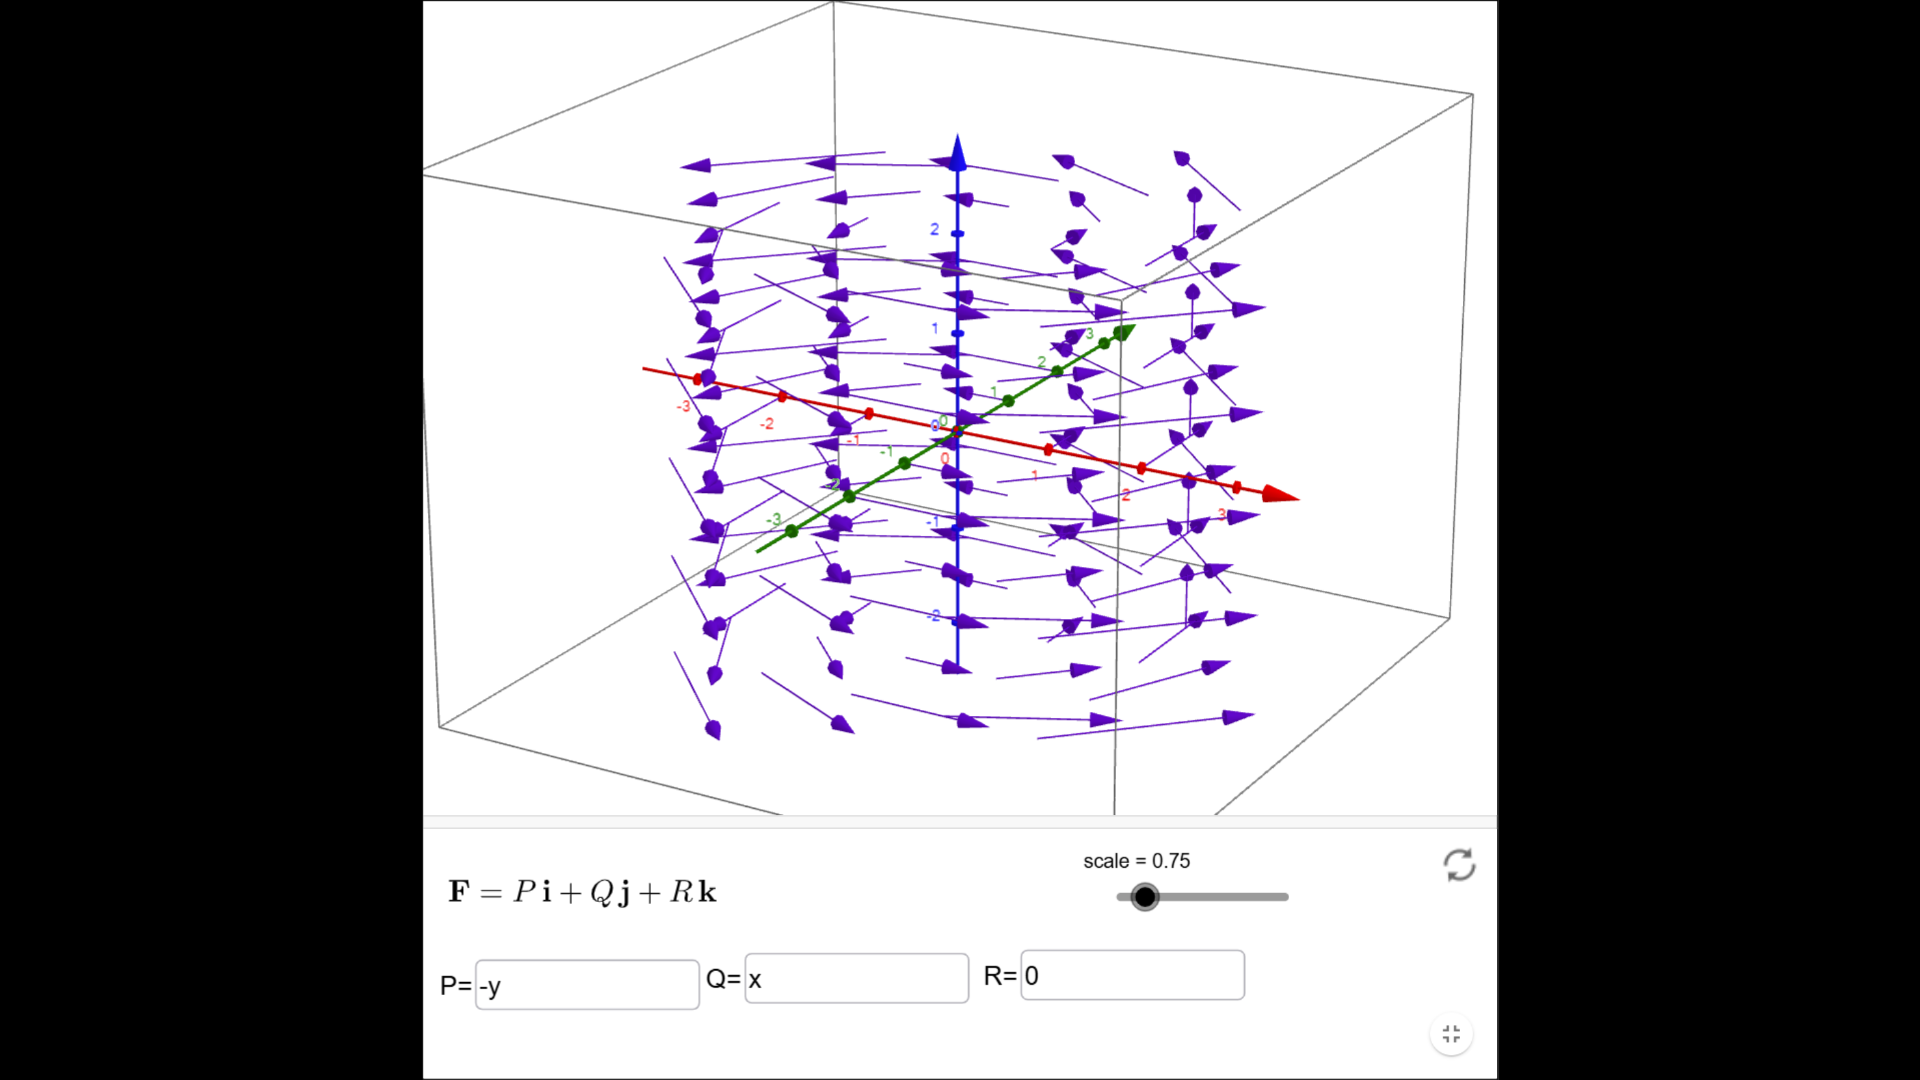
\includegraphics[width=1\linewidth]{Screenshot (315).png}
\end{figure}

\subsection{Vector Calculus Theorems}
\subsubsection{Gauss's Divergence Theorem}
Gauss's divergence theorem states that:
\begin{equation}
\iint\limits_S \vec F \cdot d\vec s = \iiint\limits_V \nabla \cdot \vec F dV
\end{equation}
In words, the flux of a vector field through a closed surface is equal to the integral of the divergence of that vector field through the volume enclosed by that surface.
\subsubsection{Stokes's Theorem}
Stokes' theorem states that:
\begin{equation}
\int_C \vec F \cdot d\vec r = \iint\limits_S \nabla \times \vec F d\vec s
\end{equation}
In words, the line integral of a vector field along a curve is equal to the surface integral of a vector field through a surface whose boundary is that curve.

You have probably also noticed that the divergence is associated with the divergence theorem and the curl is associated with Stokes's theorem.

\vspace{1em}
These theorems will allow us to switch between integral and differential forms of the equations in the derivation sections.

\subsubsection{Note on Total and Partial Derivative Usage}
You will notice in the sections for Faraday's Law and Ampére-Maxwell's Law that the integral form uses total derivatives ($\frac{d}{dt}$, while the differential form uses partial derivatives ($\frac{\partial}{\partial t}$). Why?

\vspace{1em}

For the differential forms: The electric $\vec E(\vec r, t)$ and magnetic $\vec B(\vec r, t)$ fields depend on both space/position and time. So when computing how they change with respect to time at a fixed point in space, we need to take a partial derivative. Using total derivatives would suggest either that the field is only a function of time or that we are tracking it along a specific path, neither of which are true in our cases.

\vspace{1em}

For the integral forms: But now you may be wondering why the integral forms \textit{don't} use partial derivatives! These integral forms involve total time derivatives of flux. This is because flux is already the result of an integral over space, so now we are just looking at how that scalar quantity changes over time. Let me put all of this in another way:

\vspace{1em}

In the differential form of Maxwell's equations, we are looking at how fields vary at a single point in space over time. For instance, imagine you dip a stick into the water at one point in a river, and you see how the current or water level changes just at that point over time.

\vspace{1em}
In the integral form of Maxwell's equations, we are looking at how fields vary across an entire region over time. For instance, imagine you are looking at an entire section of the river that flows through a large pipe, and you see how the amount of water that flows through the pipe changes over time.

\vspace{1em}
The differential and integral forms of Maxwell's equations describe the same physics; it's just that the differential form is "zoomed in" and the integral form is "zoomed out".

\subsection{Useful Symbols}
There are many symbols used in Maxwell's equations, and knowing what they mean is important for understanding the equations themselves. I will sometimes remind you of these symbols' meanings in the appropriate section as well. For now, here is a list:
\begin{itemize}
\item $\vec E$ : electric field
\item $\vec B$ : magnetic field
\item $\rho$ : charge density
\item $\varepsilon_0$ : permittivity of free space (constant), $8.854 \times 10^{-12} m^{-3}kg^{-1}s^4A^2$
\item $\Phi_E$ : electric flux
\item $\Phi_B$ : magnetic flux
\item $\mu_0$ : permeability of free space, $4\pi \times 10^{-7} \frac{N}{A^2}$
\item $\vec J$ : current density
\end{itemize}

\pagebreak
\section{Gauss's Law}

\iffalse 
For all of them:

Include both integral and differential forms

Show how the math relates to the physics

Use \boxed{} to spotlight key equations

\fi

By observation, we know that charged objects exert forces (a push or a pull) on each other. Then, the force on a small test charge $q_0$ is $\vec F = q_0 \vec E$, where $\vec E$ is a vector field assumed to be produced by charge. 

\vspace{1em}

If we have a point charge $q$, the electric field it produces must point away (radially outward) from the charge and have the same magnitude at equidistant points from the charge (symmetric). It should also decrease as distance from the charge increases.

(This is Coulomb's Law; it states that the electric field produced by point charge $q$ at distance $r$ is $\vec E = \frac{1}{4\pi\varepsilon_0)} \frac{q}{r^2} \hat{r}$, where $\hat{r}$ is the radial direction.)

\vspace{1em}

One thing we can do is enclose $q$ in a spherical Gaussian surface (see image below) to determine the total electric flux through that surface. In general, you can think of flux as the amount of "stuff" passing through a surface over a certain amount of time (think of water passing through a net). 

\vspace{5em}

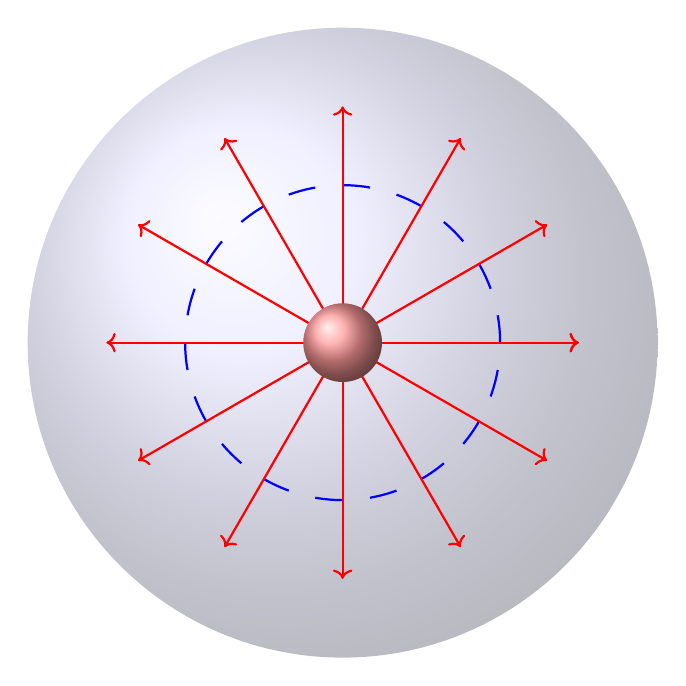
\begin{tikzpicture}
\shade[ball color=blue!20, opacity = 0.4, dashed] (0,0) circle (4cm);
\foreach \angle in {0,20,...,340} {
    \draw[blue, thick] (\angle:2cm) arc[start angle=\angle, end angle=\angle+10, radius=2cm];}

\foreach \angle in {0,30,...,360} {
    \draw[->, red, thick] (0,0) -- (\angle:3cm);
  }
\shade[ball color=red!40] (0,0) circle (0.5cm);

\end{tikzpicture}

\vspace{5em}

The total flux through the closed Gaussian surface solely depends on the charge inside. So, we can define the electric flux to be:
\begin{equation}
\boxed{\Phi_E = \oint_{S} \vec E \cdot \, d\vec A = \frac{Q_{enc}}{\varepsilon_0}}
\end{equation}
where $\varepsilon_0$ is an experimentally-determined constant. This is the integral form of Gauss's Law.

\vspace{1em}

Instead of a point charge, what if we had a continuous distribution of charge enclosed within a Gaussian surface? Then, the enclosed charge would instead be $Q_{enc} = \int_{V} \rho(r) dV$, where $\rho$ is charge density as a function of distance. Therefore, our equation for Gauss's Law becomes:
\begin{equation}
\Phi_E = \oint_{S} \vec E \cdot \, d\vec A = \frac{1}{\varepsilon_0}\int_{V} \rho(r) dV
\end{equation}
Now we can use Gauss's Divergence Theorem to rewrite the surface integral in terms of a volume integral:
\begin{equation}
\Phi_E = \int_{V} \nabla \cdot \vec E \, dV = \frac{1}{\varepsilon_0}\int_{V} \rho(r) dV
\end{equation}
and therefore:
\begin{equation}
\boxed{\Phi_E = \nabla \cdot \vec E \, = \frac{\rho}{\varepsilon_0}}
\end{equation}
This is the differential form of Gauss's Law.

\pagebreak
\section{Gauss's Law for Magnetism}
\iffalse
Emphasize the absence of magnetic monopoles.

Show field lines looping back on themselves.

Use closed surfaces to explain why total flux is always zero.
\fi

From experiments like Oersted's discovery that a compass needle deflects when placed near a current-carrying wire, we know that electric currents (moving electric charges) generate magnetic fields. We also know from this that magnetic fields actually exist. Let us use $\vec B$ to represent this vector field generated by magnetic effects.

\vspace{1em}

%Also, mention Biot-Savart law; can derive Gauss's for Magnetism from this law.

We can use reasoning similar to the reasoning we used for Coulomb's Law here to better understand how magnetic fields are generated by currents. Recall from the previous discussion on Coulomb's Law that a stationary point charge $q$ produces an electric field pointing radially outward that decreases as distance increases (proportional to $\frac{1}{r^2}$). Analogously, a small segment of current-carrying wire (moving charge) should produce a magnetic field with a similar relationship to distance. However, experiments such as Oersted's show that the direction of the magnetic field is not radially outward but rather circulatory (looping around the wire).

All this suggests that the magnetic field must be proportional to the current, proportional to $\frac{1}{r^2}$, and point in a direction \textit{perpendicular to both the direction of the current $d\vec l$ and the direction of the position vector}. That italicized requirement tells us that we need to use a cross product here! 

These considerations lead to:
\begin{equation}
d\vec B = \frac{\mu_0}{4\pi} \frac{I\, d\vec l \times \hat r}{r^2}
\end{equation}

This is the Biot-Savart Law (the total magnetic field can be found by integration). Note that a magnetic field generated this way always curls around the source of current and has no divergence— this will be directly applicable when deriving Gauss's Law for Magnetism.

(The magnitude of $d \vec B$ is $dB = \frac{\mu_0}{4\pi} \frac{I\, dl sin\theta}{r^2}$, and the direction follows the right-hand rule).

\vspace{1em}

By mapping out fields for different current configurations using small test objects, we find that the magnetic field lines always connect in loops (see image below). Therefore, if we think about the magnetic "flow", we can say that the entering and exiting "flows" are equal.

\vspace{3em}

\begin{figure}[H]
    \centering
    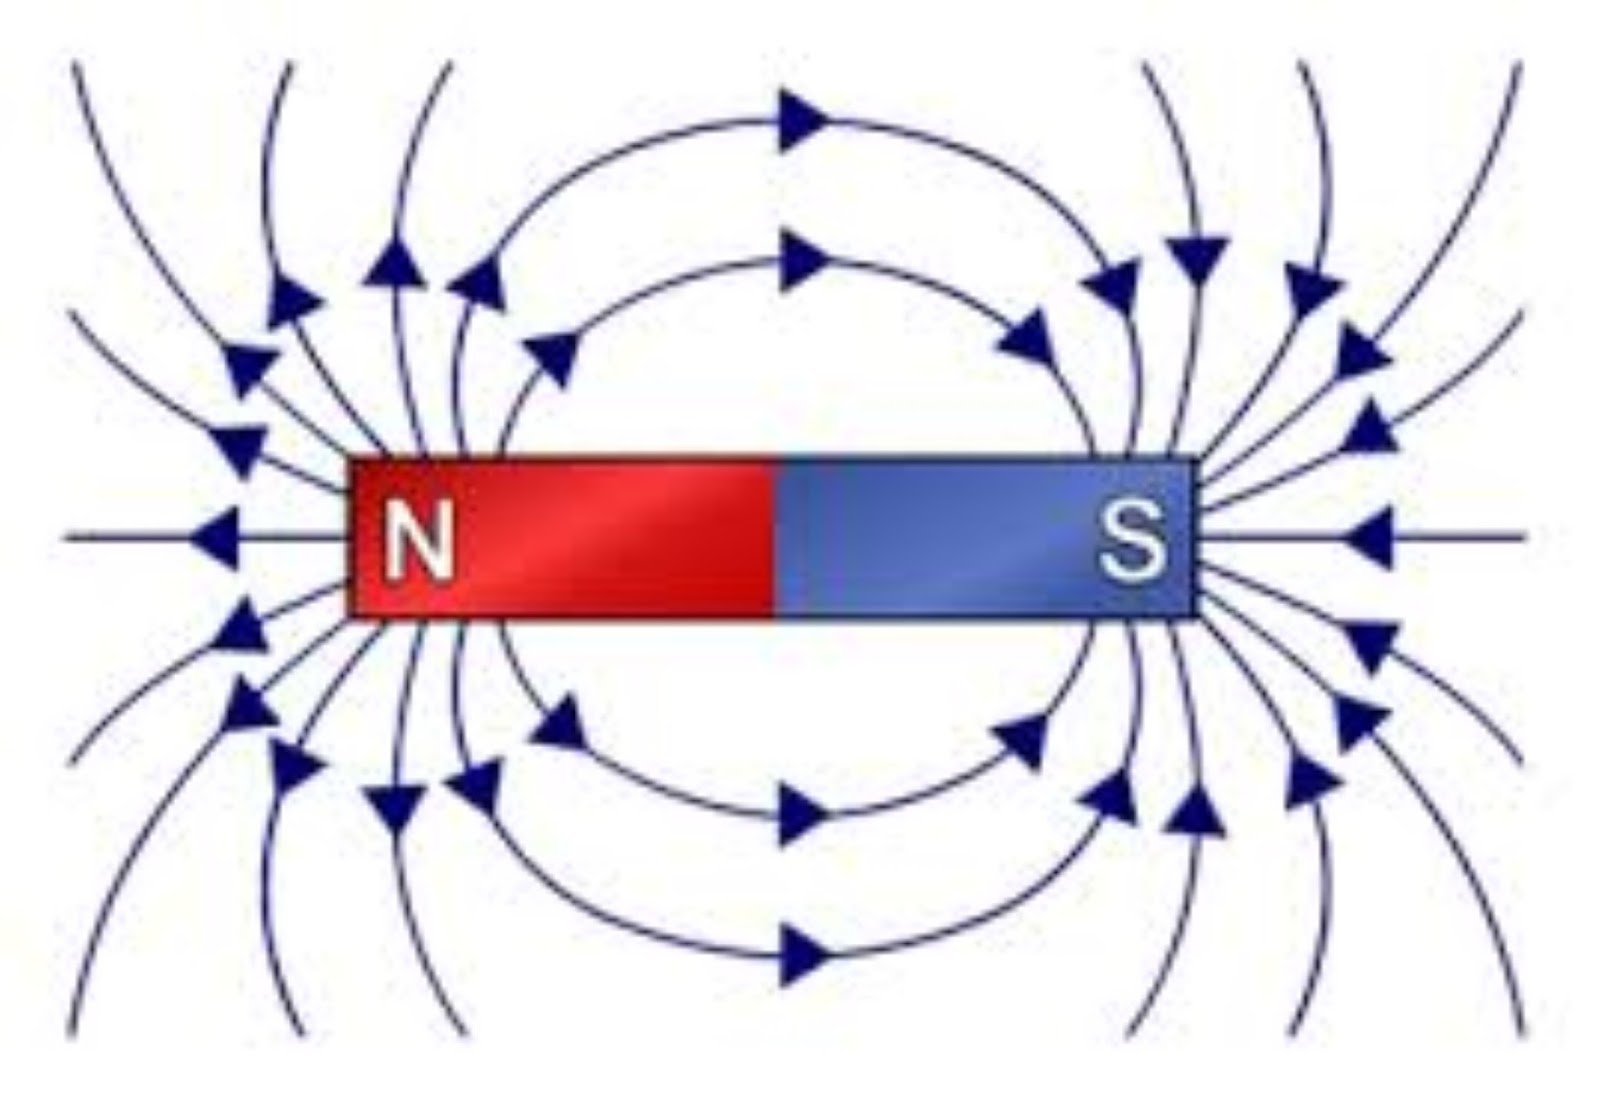
\includegraphics[width=0.5\linewidth]{barmagnet.png}
    %\caption{Enter Caption}
    %\label{fig:enter-label}
\end{figure}

\vspace{3em}

We might ask whether there \textit{is} ever any net magnetic field flowing out of some region in space. To find out, we can enclose a magnetic source, such as a bar magnet or loop of current-carrying wire, in a Gaussian surface to determine the total magnetic flux through the surface. However, since magnetic fields loop around the source, any field line that exits the Gaussian surface at some point must also loop around and re-enter the surface at some other point. This observed symmetry implies that magnetic monopoles (i.e. isolated sources of magnetism) do not exist. All this is to say that the magnetic flux can be defined as:

\begin{equation}
\boxed{\Phi_B = \oint_S \vec B \cdot d\vec A = 0}
\end{equation}
This is the integral form of Gauss's Law for Magnetism.

\vspace{1em}
Now we can use Gauss's Divergence Theorem to rewrite the surface integral in terms of a volume integral:
\begin{equation}
\phi_B = \int_V \nabla \cdot \vec B dV = 0
\end{equation}
Since this relation must hold for any arbitrary volume V, the integrand itself must be equal to 0. Therefore:
\begin{equation}
\boxed{\phi_B = \nabla \cdot \vec B = 0}
\end{equation}
This is the differential form of Gauss's Law for Magnetism.

\pagebreak
\section{Faraday's Law}
\iffalse
Introduce a changing magnetic flux in a loop.

Use Stokes’ Theorem to relate loop integral to curl.

Illustrate with induced electric field loops and animation-style TikZ visuals.
\fi

In 1831, Faraday observed that when a magnet is moved through a loop of wire, a current is detected. Furthermore, when the magnet stopped, the current stopped, and when the magnet was reversed so was the direction of current. So, the current was not caused solely by the magnet's existence, but by the fact that the magnetic field was changing over time (because the magnet was moving). In other words, a changing magnetic field induces current.

\vspace{1em}

Faraday realized that a changing magnetic flux within this loop of wire created a voltage through the circuit without the need of a battery. This induced voltage is also called electromotive force, or emf ($\epsilon$. Therefore:
\begin{equation}
\epsilon = -\frac{d\phi_B}{dt}
\end{equation}

\vspace{1em}
This law is known as Lenz's Law because Lenz figured out the minus sign. The minus sign is there because the emf tries to resist change in the magnetic flux (see image below).

\vspace{3em}
\begin{figure}[h]
    \centering
    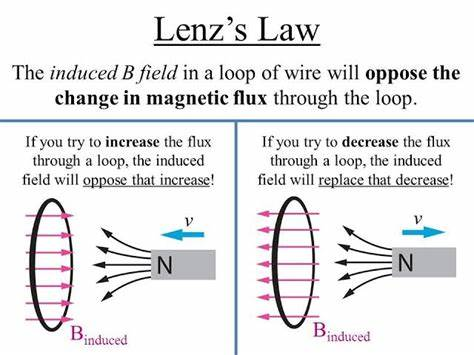
\includegraphics[width=0.7\linewidth]{LenzDiagram.png}
\end{figure}
\vspace{3em}

\vspace{1em}
For a continuous magnetic field, the magnetic flux can be written as 
\begin{equation}
\phi_B = \int_S \vec B(t) d\vec A
\end{equation} 

\vspace{1em}
Recall that voltage is defined to be the potential difference per unit of charge between two points in an electric field. Also, the total emf is equal to the sum of the emfs at each point in the circuit. So, the total emf is equal to the sum of the electric field at each point of the circuit. Say we have a loop of wire (a curve) with length L. Then:

\begin{equation}
\boxed{\epsilon = -\frac{d}{dt}\int_S \vec B \cdot d \vec A = \oint_C \vec E \cdot d \vec L}
\end{equation}

\vspace{1em}
This is the integral form of Faraday's Law.

Now we can use Stokes' Theorem to rewrite the integral over a curve in terms of a surface integral:

\begin{equation}
\epsilon = -\frac{d}{dt}\int_S \vec B \cdot d \vec A = \int_S \nabla \times \vec E d\vec A
\end{equation}

and therefore:
\begin{equation}
\boxed{\epsilon = -\frac{\partial \vec B}{\partial t} = \nabla \times \vec E}
\end{equation}
This is the differential form of Faraday's Law.

\pagebreak
\section{Ampère-Maxwell Law}

\iffalse
Begin with Ampère’s circuital law.

Introduce displacement current concept via charging capacitor.

Use Stokes’ Theorem again.

Show magnetic field circles around current and growing electric field.
\fi
From experiments such as Oersted's, we know that a current-carrying wire (steady current) results in a magnetic field that loops around the wire. So, the sum of all the magnetic fields around the loop (a curve) should be proportional to the enclosed current. Taking a proportionality constant $\mu_0$:

\begin{equation}
\oint_C \vec B \cdot d\vec l = \mu_0 I_{enc}
\end{equation}

This is Ampère's Law, and works for steady current. 

However, we are not done!

\vspace{1em}
Imagine a simple circuit containing a battery, wires, and a capacitor. A capacitor can be thought of as a gap in the circuit, since the two plates are not touching. Therefore, as the capacitor charges, although current flows in the wire no actual charge crosses between the gap in the plates. The electric field is also rapidly changing as the capacitor charges. However, a magnetic field is observed! There must be another kind of current between the plates. In its original form, Ampère’s Law is not enough to explain the behavior of time-varying electric fields in capacitors.

\vspace{3em}
\begin{center}
\begin{circuitikz}

\fill[green!20] (4,1) circle (0.3); %fill for Gaussian surface

  \draw[->, thick, black] (0.2,0) -- (3.8,0);% Arrow at the bottom wire
  \draw[->, thick, black] (4,0.2) -- (4,1.8); % Right side (through capacitor)
  \draw[->, thick, black] (3.8,2) -- (0.2,2); % Top wire
  \draw[->, thick, black] (0,1.8) -- (0,0.2); % Left side (through battery)

  \draw (0,0)
        to[battery1, l_=$V$] (0,2)
        to[short] (4,2)
        to[C=$C$] (4,0)
        to[short] (0,0);

  \draw[ ->, red] (4,0.9) -- (4,1.1);
  \draw[->, red] (3.6,0.9) -- (3.6, 1.1);
  \draw[->, red] (4.4, 0.9) -- (4.4, 1.1);

%magnetic field line
 \draw[->, blue, dashed] (4,1) circle (0.2);

%gaussian surface boundary
\draw[dotted, thick, green] (4,1) circle (0.3);
\end{circuitikz}
\end{center}

\vspace{1em}
(In this image, the red arrows represent the electric field lines that must be present between the plates of the capacitor. The blue loop represents the magnetic field observed. The green shaded area represents a Gaussian surface between the plates of the capacitor, and the black arrows throughout the circuit represent the direction of conventional current flow.)
\vspace{1em}

So, Maxwell proposed a new kind of "current" made not of moving charges but of changing electric fields. The electric field between the plates of a capacitor increases as the charge increases:
\begin{equation}
\Phi_E = \oint_S \vec E \cdot d\vec A
\end{equation}
Recall that this was our definition of electric flux. If the electric field is changing, the electric flux is a non-zero value. Maxwell said that this change in flux contributed to the magnetic field as well. He defined the \textit{displacement current} as:
\begin{equation}
I_d = \varepsilon_0 \frac{d\phi_E}{dt}
\end{equation}

And therefore, the extended Ampère's Law becomes:
\begin{equation}
\boxed{\oint_{C} \vec B \cdot d\vec l = \mu_0 ( I_{enc} + \varepsilon_0 \frac{d}{dt}\int_S \vec E \cdot d\vec A )}
\end{equation}
This is the integral form of Ampère-Maxwell's Law.

Now we can use Stokes' Theorem to rewire the integral over a curve in terms of a surface integral:
\begin{equation}
\int_S \nabla \times \vec Bd\vec A = \mu_0 ( I_{enc} + \varepsilon_0 \frac{d}{dt}\int_S \vec E \cdot d\vec A )
\end{equation}

Expanding out the right-hand side and solving:

\begin{equation}
\boxed{\nabla \times \vec B = \mu_0\vec J + \mu_0\varepsilon_0 \frac{\partial\vec E}{\partial t}}
\end{equation}

This is the differential form of Ampère-Maxwell's Law, where $\vec J$ is current density.

\pagebreak
\section{Conclusion}

\iffalse 
Reflect on what the equations unify and how they form the backbone of classical electromagnetism.

Optional: Comment on how these equations set the stage for relativity or wave theory.
\fi

Through the process of deriving Maxwell's equations from first principles, we can gain a clearer understanding on how electric and magnetic fields interact. Each equation came from a combination of experimental evidence backed by formal mathematics such as Gauss's Divergence Theorem and Stokes's Theorem. Visualizing the vector fields and translating that into both integral and differential forms help us see how these equations also symbolize a geometric aspect in space.

\vspace{1em}
Maxwell’s equations not only unify electric and magnetic phenomena but also serve as the foundation for many areas of modern physics and engineering. When combined in a region free of electric field or magnetic field sources (charge density and current density are both 0), these equations predict that electric and magnetic fields can still propagate together as waves through space—electromagnetic waves—with speed $ c = \frac{1}{\sqrt{\mu_0 \varepsilon_0}} = 2.998 \times 10^8 m/s $. This result led to the statement that light is an electromagnetic wave, and linked optics to electromagnetism.

%https://en.wikipedia.org/wiki/Electromagnetic_wave_equation

\vspace{1em}
Additionally, the symmetry and structure of these equations laid the foundations for Einstein's theories of relativity. The fact that the speed of electromagnetic waves is constant in all inertial reference frames raised questions about how time and space actually behave.

\vspace{1em}
In a more practical sense, Maxwell's equations have helped shape the development of numerous modern technologies including wireless communication, radar, television, and medical imaging equipment. All of them rely on the principles detailed in these four compact equations.

\vspace{5em}

\begin{center}
\textbf{Maxwell's Equations}
\end{center}
\renewcommand{\arraystretch}{2.2}
\begin{center}
\fbox{%
\begin{tabular}{lcl}
\textbf{Integral Form} &  & \textbf{Differential Form} \\
$\oint_S \vec{E} \cdot d\vec{A} = \dfrac{Q_{\text{in}}}{\varepsilon_0}$ & & $\nabla \cdot \vec{E} = \dfrac{\rho}{\varepsilon_0}$ \\
$\oint_S \vec{B} \cdot d\vec{A} = 0$ & & $\nabla \cdot \vec{B} = 0$ \\
$\oint_{C} \vec{E} \cdot d\vec{l} = -\dfrac{d\phi_B}{dt}$ & & $\nabla \times \vec{E} = -\dfrac{\partial \vec{B}}{\partial t}$ \\
$\oint_{C} \vec{B} \cdot d\vec{l} = \mu_0 I_{\text{enc}} + \mu_0 \varepsilon_0 \dfrac{d\phi_E}{dt}$ & & $\nabla \times \vec{B} = \mu_0 \vec{J} + \mu_0 \varepsilon_0 \dfrac{\partial \vec{E}}{\partial t}$ \\
\end{tabular}
}%
\end{center}
\end{document}
